% This file was created by matplotlib2tikz v0.7.4.
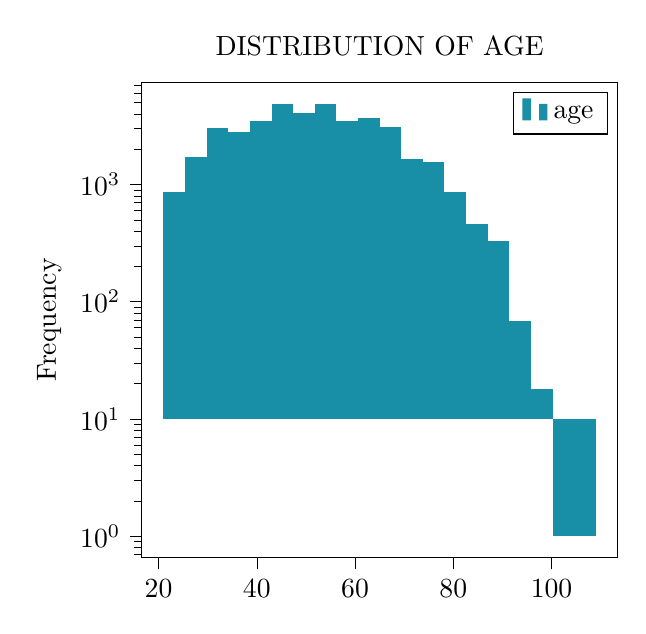
\begin{tikzpicture}

\definecolor{color0}{rgb}{0.0941176470588235,0.56078431372549,0.654901960784314}

\begin{axis}[
height=3in,
log basis y={10},
tick align=outside,
tick pos=left,
title={\printsubsection{\MakeUppercase{Distribution of age}}\\},
width=3in,
x grid style={white!69.01960784313725!black},
xmin=16.6, xmax=113.4,
xtick style={color=black},
y grid style={white!69.01960784313725!black},
ylabel={Frequency},
ymin=0.653928276154919, ymax=7479.41353562344,
ymode=log,
ytick style={color=black}
]
\draw[fill=color0,draw opacity=0] (axis cs:21,0) rectangle (axis cs:25.4,860);
\addlegendimage{ybar,ybar legend,fill=color0,draw opacity=0};
\addlegendentry{age}

\draw[fill=color0,draw opacity=0] (axis cs:25.4,0) rectangle (axis cs:29.8,1725);
\draw[fill=color0,draw opacity=0] (axis cs:29.8,0) rectangle (axis cs:34.2,3033);
\draw[fill=color0,draw opacity=0] (axis cs:34.2,0) rectangle (axis cs:38.6,2801);
\draw[fill=color0,draw opacity=0] (axis cs:38.6,0) rectangle (axis cs:43,3519);
\draw[fill=color0,draw opacity=0] (axis cs:43,0) rectangle (axis cs:47.4,4856);
\draw[fill=color0,draw opacity=0] (axis cs:47.4,0) rectangle (axis cs:51.8,4093);
\draw[fill=color0,draw opacity=0] (axis cs:51.8,0) rectangle (axis cs:56.2,4891);
\draw[fill=color0,draw opacity=0] (axis cs:56.2,0) rectangle (axis cs:60.6,3520);
\draw[fill=color0,draw opacity=0] (axis cs:60.6,0) rectangle (axis cs:65,3677);
\draw[fill=color0,draw opacity=0] (axis cs:65,0) rectangle (axis cs:69.4,3073);
\draw[fill=color0,draw opacity=0] (axis cs:69.4,0) rectangle (axis cs:73.8,1651);
\draw[fill=color0,draw opacity=0] (axis cs:73.8,0) rectangle (axis cs:78.2,1569);
\draw[fill=color0,draw opacity=0] (axis cs:78.2,0) rectangle (axis cs:82.6,867);
\draw[fill=color0,draw opacity=0] (axis cs:82.6,0) rectangle (axis cs:87,460);
\draw[fill=color0,draw opacity=0] (axis cs:87,0) rectangle (axis cs:91.4,333);
\draw[fill=color0,draw opacity=0] (axis cs:91.4,0) rectangle (axis cs:95.8,68);
\draw[fill=color0,draw opacity=0] (axis cs:95.8,0) rectangle (axis cs:100.2,18);
\draw[fill=color0,draw opacity=0] (axis cs:100.2,0) rectangle (axis cs:104.6,1);
\draw[fill=color0,draw opacity=0] (axis cs:104.6,0) rectangle (axis cs:109,1);
\end{axis}

\end{tikzpicture}